\documentclass[10pt,a4paper]{article}
\usepackage[utf8]{inputenc}
\usepackage[italian]{babel}
\usepackage{amsmath}
\usepackage{amsfonts}
\usepackage{amssymb}
\usepackage{graphicx}
\usepackage{gensymb}
\usepackage[left=2cm,right=2cm,top=2cm,bottom=2cm]{geometry}
\newcommand{\rem}[1]{[\emph{#1}]}

\author{Gruppo BN \\Lisa Bedini,  Federico Belliardo, Marco Costa}
\title{Esperienza 15: Misura della costante di Boltzmann}
%TODO diminuire dimensione foto oscilloscopio e aumentare quella dei grafici
\begin{document}
\maketitle
\section{Scopo dell'esperienza}
Misurare la costante di Boltzmann dal rumore termico (Johnson-Nyquist) di una resistenza a temperatura nota, grazie ad un amplificatore, un filtro passa-banda e un convertitore RMS.

\section{Materiale a disposizione}
\begin{itemize}
\item INA114 Amplificatore
\item AD708: OpAmp integrati
\item AD736: RMS converter
\end{itemize}

%TO DO: l'errore sul voltaggio in uscita è stato preso come sedmidispersione dell'oscillazione
Tutte le resistenze, i condensatori, le tensioni di alimentazione sono stati misurati con il multimetro digitale (in DC), quindi l'errore è stato propagato secondo le specifiche nel manuale ($0.8\% + 3\,\mbox{digit}$ per le resistenze,$4\% + 3\, \mbox{digit}$  per i condensatori, $0.5\% + 1\,\mbox{digit}$ per i voltaggi).
Date le fluttuazioni dei valori della tensione in uscita,  per queste l'errore è stato stimato come semidispersione rispetto al valore centrale. I tempi e le restanti tensioni sono state misurate con i cursori dell'oscilloscopio: l'errore sui tempi è dato dalla risoluzione dei cursori stessi mentre quello sulle tensioni è stato propagato considerando solamente l'errore sul posizionamento dei cursori. E' stato trascurato l'errore sistematico del $3\%$ dell'oscilloscopio nella misure di tensione poiché queste compaiono solo in rapporti e la componente sistematica tende a compensarsi.

%TODO Dire come si sono propagati gli errori in tutta l'esperienza: Nei bode l'errore non è stato proprio considerato questa cosa è tecnicamente sbagliata ma venivano orribili se li consideravo, non scrivere. In rutti gli altri l'errore è stato propagato statistico.
%TODO Forse dovrei aggiungere qualcosa su come si sono propagati gli errori, di fatto l'unica formula in cui propago arrori è l'ultima per kb e ho detto che si sono propagati in quadratura. Ripeto nei bode non considero l'errore. NEl fit di Boltzmann considero l'errore solo sulle tensioni.

\section{Montaggio del circuito}
\subsection{Power filter}
La tensione di alimentazione (positive e negative) sono state filtrate mediante circuiti passa-basso (figura \ref{power}) prima di fornirle agli integrati in modo da ridurne le fluttuazioni:

\begin{figure}[!htb]
\centering
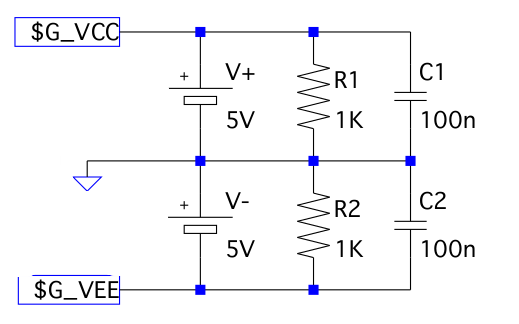
\includegraphics[scale=0.5]{powerfilter.png}
\caption{Filtri passa basso per le alimentazioni.\label{power}}
\end{figure}


\subsection{Preamplificatore}
%TODO Ho buttato via il foglio con i valori giusti isurati se no avrei fatto il calcolo con quelli in vece che con i valori nominali...
Abbiamo montato il circuito in figura \ref{preamp}.
Il primo stadio di amplificazione è stato realizzato con un \emph{Precision instrumentation amplifier} avente un guadagno atteso: $G_1 = 1+\frac{50 k\Omega}{1 k\Omega} = 51$. Il secondo stadio è un semplice amplificatore invertente con guadagno teorico $G_2 = \frac{68 k\Omega}{4.7 k\Omega} = 14.5$. Il valore atteso dell'amplificazione complessiva è: $A_1 = 740$, dove abbiamo moltiplicato le due amplificazioni: le resistenze in ingresso dei due circuiti sono grandi rispetto a quelle in uscita.

%Questa è la tipica frase che fa perdere punti. In che senso?
%Non sono stati propagati gli errori sulle resistenze per stimare l'incertezza sul %guadagno teorico. Si nota che anche volendo farlo non conosciamo la precisione sulla %calibrazione della resistenza interna dall'INA114.\\

\begin{figure}[!htb]
\centering
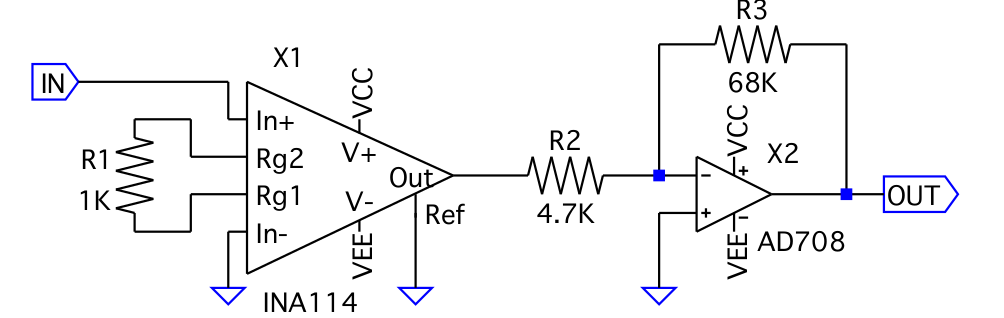
\includegraphics[scale=0.5]{preamp.png}
\caption{Preamplificatore realizzato con OpAmp AD708 e INA114.\label{preamp}}
\end{figure}

%TODO Parlare di come è fatto dentro l'INA (sono 3 opAmp)?

Per limitare il rumore tutte le terre di uno stesso "blocchetto" della breadboard sono state collegate ai "blocchetti" adiacenti. Sono state collegate anche le due linee di terra usate in modo trasversale alla linea stessa. In questo modo si sono evitati offset spuri nel circuito. %ditemi se vi piace la frase.

Il circuito è stato analizzato fornendo in ingresso con il generatore di funzioni un onda sinusoidale di piccola ampiezza ($V_0 = 7.1 \pm 0.1$mV picco-picco) e misurando l'ampiezza picco picco del segnale in uscita. L'ampiezza del segnale in ingresso è stata scelta come la più alta possibile che non mandasse in saturazione l'opAmp a bassa frequenza, ossia nella zona dove è atteso il guadagno massimo. L'ingresso è prima dell'integrato INA114 e l'uscita dopo l'amplificatore invertente. %frase forse ridondante
I dati raccolti sono in tabella \ref{tabellaBode1} e riportati nel diagramma di bode in figura \ref{bode}.
Si è eseguito un fit (con la funzione \emph{curve fit} di \emph{pylab})con la funzione di trasferimento di un integratore: $A(\omega) = \frac{A_1}{\sqrt{1+\left( \frac{f}{f_t} \right) }}$. Da questo si vede che il preAmp si comporta effettivamente come un filtro passa basso con una frequenza di taglio $f_t = 14 \pm 1$kHz e un'ampiezza massima $A_{1} = 770 \pm 10$, che è maggiore di quella attesa poiché le resistenze reali hanno un valore leggermente diverso da quello di progettazione. La matrice di covarianza\footnote{In tutta la relazione non si sono mai riportate le unità di misura delle entrate della matrice di covarianza, poiché sono le ovvie combinazioni delle unità in cui sono stati riportati i dati numerici: in questo caso $mV$ e $\mbox{kHz}$.} è: $\Sigma_{ij} = \left( \begin{array}{cc}
1.02 & -7.00\\ 
-7.00 & 167\\
\end{array} \right)$. Con un $\chi^2/ndof = 114/10$.

\begin{table}[!htb]\centering
\begin{tabular}{|c|c|c|c|}
\hline
$V_{out} (mV)$ & $\Delta V_{out} (mV)$ & $f (\mbox{kHz})$ & $\Delta f (\mbox{kHz})$\\ 
\hline
5.36 & 0.04 & 0.00098 & 0.00001\\
5.36 & 0.04 & 0.0097 & 0.0001\\
5.36 & 0.04 & 0.098 & 0.001\\
5.36 & 0.04 & 0.99 & 0.01\\
5.36 & 0.04 & 3.00 & 0.03\\
5.36 & 0.04 & 5.98 & 0.06\\
4.96 & 0.04 & 10.0 & 0.1\\
4.24 & 0.04 & 14.8 & 0.1\\
3.48 & 0.04 & 20.1 & 0.2\\
2.84 & 0.02 & 25.5 & 0.3\\
1.37 & 0.02 & 49.7 & 0.5\\
0.52 & 0.01 & 100 & 1\\
\hline
\end{tabular}
\caption{Tensioni in uscita dal preamplificatore $V_{out}$ in funzione della frequenza $f$.}
\label{tabellaBode1}
\end{table}

\begin{figure}[!htb]
\centering
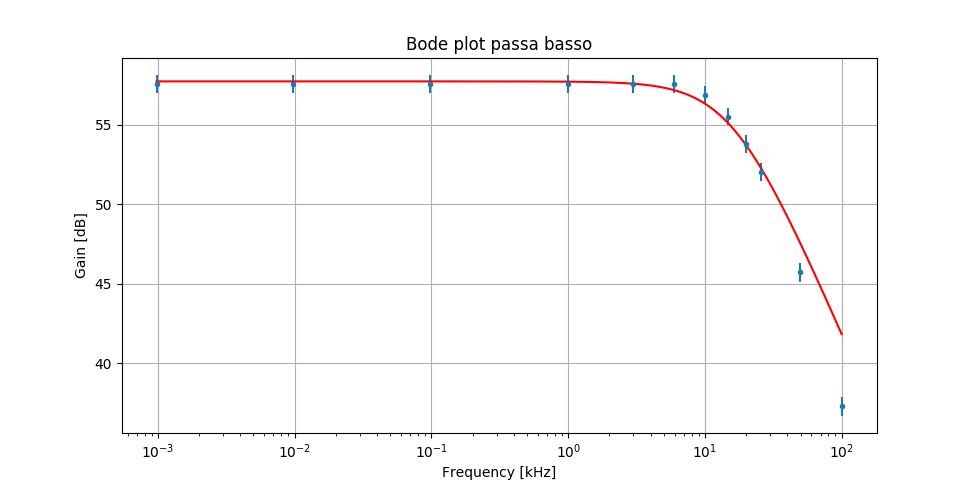
\includegraphics[scale=.7]{bodeBasso.png}
\caption{Diagramma di Bode del preamplifiatore.\label{bode}}
\end{figure}

%TODO Non ha più alcun senso
%accorgimento per l'offset
%L'offset del generatore di funzioni è stato modificato finemente in modo che il segnale in uscita fosse il %più possibile a media nulla. L'offset residuo è dell'ordine del mV. Questo segnale in continua viene %amplificato fino ad avere un segnale dell'ordine dei volt di offset sull'uscita. Le misure eseguite sono %comunque picco-picco quindi l'offset non ha alcuna influenza (se il circuito lavora in regime lineare).\\
%Altra frase da evitare
%Abbiamo usato accoppiamento AC dell'oscilloscopio

Per frequenze basse si vede in figura \ref{integratoreBasso} che il circuito agisce da amplificatore e esegue uno sfasamento del segnale di $\pi \, rad$. Infatti l'integrato che funziona da passa-basso aggiunge una fase nulla ed è l'amplificatore invertente che sfasa il segnale. Alle alte frequenze (figura \ref{integratoreAlto}) l'integratore sfasa di $-\frac{\pi}{2}$, dunque lo sfasamento complessivo è $\frac{\pi}{2}$ e il segnale di uscita è anticipato.

\begin{figure}[!htb]
\centering
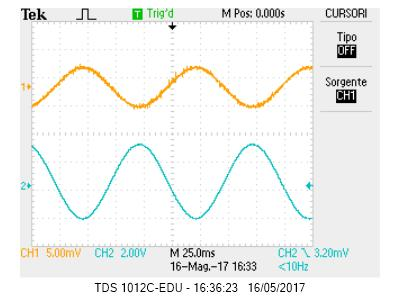
\includegraphics[scale=1.0]{integratoreBassaFrequenza.jpg}
\caption{Onde sfasate di $\pi$ rad in ingresso e uscita al preamplificatore.\label{integratoreBasso}}
\end{figure}

\begin{figure}[!htb]
\centering
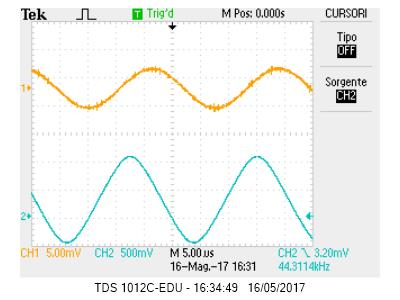
\includegraphics[scale=1.0]{integratoreAltaFreq.jpg}
\caption{Onde sfasate di $\frac{\pi}{2}$ rad in ingresso e uscita al preamplificatore.\label{integratoreAlto}}
\end{figure}

Si vede che alle alte frequenze l'attenuazione per decade è maggiore di quella attesa di $20\frac{dB}{decade}$. Questo è compatibile con la presenza di ulteriori poli che diventano importanti ad alta frequenza all'interno dell'OpAmp. La deviazione dalla legge attesa (che rappresenta un andamento non solamente un errore sperimentale) è la causa del $\chi^2$ fuori misura.

In realtà ai fini della misura del solo guadagno massimo è più efficace eseguire un fit alla sola retta dai dati a bassa frequenza, cioè dei primi sei punti con valori tutti uguali di $V_{out}$, ciò corrisponde a eseguire la semplice divisione con propagazione dell'errore che fornisce $A_1 = 754 \pm 12$.

\subsection{Filtro passa-banda e postamplificatore}
Si sono realizzati il filtro passa-banda e il postamplificatore come mostrato nelle figure \ref{banda} e \ref{postamp} rispettivamente.

\begin{figure}[!htb]
\centering
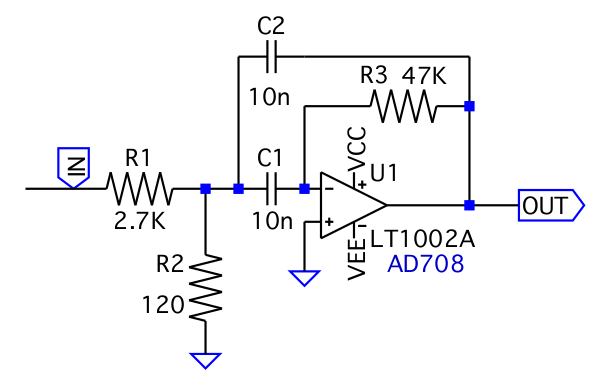
\includegraphics[scale=0.5]{banda.png}
\caption{Filtro passa-banda realizzato con OpAmp.\label{banda}}
\end{figure}


\begin{figure}[!htb]
\centering
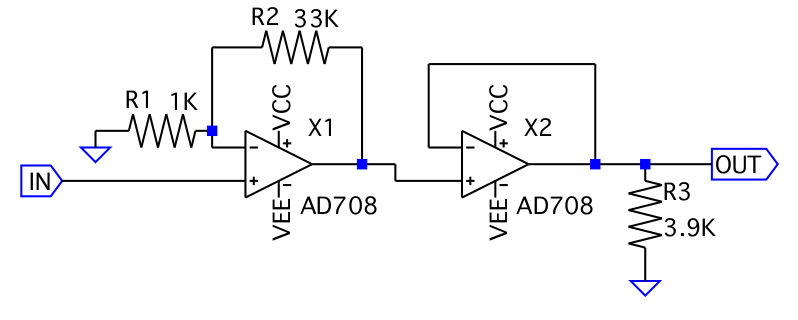
\includegraphics[scale=0.5]{postamp.png}
\caption{Postamplificatore realizzato con OpAmp.\label{postamp}}
\end{figure}

L'analisi teorica del circuito passa-banda indica che questo ha una amplificazione massima $A_{banda} = \frac{R_3}{2 R_1} = 8.7$ in corrispondenza della frequenza $f_t = \frac{1}{2 \pi C} \sqrt{\frac{\frac{1}{R_1} + \frac{1}{R_2}}{R_3}} = 6.7 \mbox{kHz}$. %errori si mettono?
La larghezza di banda prevista è: $\Delta f = \frac{1}{\pi R_3 C} = 667$Hz, agli estremi della quale l'amplificazione è di $3 dB$ inferiore a quella di picco. Il postamplificatore ha invece un guadagno $A_{post} = 1 + \frac{R_2}{R_1} = 34$, come è ben noto. L'amplificazione a centro banda attesa è dunque $A_{2} = A_{banda} A_{post} = 269$.
%TODO Piccolo sforzo per unificare le notazioni in fatto di ampiezze. Stimare errore su banda passante

L'analisi in frequenza (e la costruzione del relativo diagramma di Bode) è stata eseguita con un segnale sinusoidale di ampiezza picco-picco $V_{in} = 28.6 \pm 0.5$ mV. Abbiamo scelto questa ampiezza come la massima possibile che non mandi in saturazione gli OpAmp. L'ingresso è prima del passa-banda e l'uscita è dopo il postamplificatore. I dati sono riportati in tabella \ref{tabellaBode2}.
E' stato eseguito un fit (figura \ref{bandaFit}) a tre parametri della funzione $A(f) = \frac{A_2 \Delta f}{\sqrt{(f^2-f_0^2)^2+f \Delta f}}$, ottenuta dal modello teorico con il principio della massa virtuale. Esso ha riportato come risultati: $A_2 = 235.6 \pm 1.2$, $f_0 = 6.349 \pm 0.002$kHz, $\Delta f = 638 \pm 6$Hz. La matrice di covarianza risulta essere: $ \Sigma_{ij} = \left( \begin{array}{ccc}
1.34 & -2.93 \cdot 10^{-4} & -5.68 \cdot 10^{-3}\\ 
-2.93 \cdot 10^{-4} & 5.55 \cdot 10^{-4} & 1.36 \cdot 10^{-6}\\
-5.68 \cdot 10^{-3} & 1.36 \cdot 10^{-6} & 3.64 \cdot 10^{-5}\\
\end{array} \right)$. Con un $\chi^2/ndof = 136/22$.\\
Nuovamente il $\chi^2$ elevato è dovuto al fatto che ad alte frequenze l'andamento è apprezzabilmente diverso da quello \emph{fittato}.

%TODO Notare che non riporto mai le unità di misura per la matrice di covarianza per non appesantire la notazione. Sono quelle ovvie

%TODO Non sono in ordine ma non importa a nessuno. Le ordino io in freq.
\begin{table}[!htb]\centering
\begin{tabular}{|c|c|c|c|}
\hline
$V_{out} (mV)$ & $\Delta V_{out} (mV)$ & $f (\mbox{kHz})$ & $\Delta f (\mbox{kHz})$\\ 
\hline
0.011 & 0.005 & 0.098 & 0.001\\
0.0344 & 0.0005 & 0.300 & 0.003\\
0.118 & 0.004 & 1.00 & 0.01\\
0.160 & 0.004 & 1.31 & 0.01\\
0.19 & 0.01 & 1.59 & 0.02\\
0.340 & 0.008 & 2.50 & 0.03\\
0.564 & 0.008 & 3.50 & 0.04\\
1.03 & 0.02 & 4.60 & 0.05\\
1.41 & 0.02 & 5.00 & 0.05\\
2.48 & 0.04 & 5.60 & 0.06\\
3.06 & 0.08 & 5.75 & 0.06\\
4.40 & 0.08 & 5.99 & 0.06\\
5.92 & 0.08 & 6.18 & 0.06\\
6.48 & 0.08 & 6.43 & 0.06\\
5.56 & 0.08 & 6.58 & 0.07\\
3.80 & 0.08 & 6.83 & 0.07\\
2.92 & 0.04 & 7.05 & 0.07\\
2.38 & 0.08 & 7.25 & 0.07\\
1.88 & 0.04 & 7.50 & 0.07\\
1.37 & 0.02 & 8.00 & 0.08\\
1.07 & 0.02 & 8.54 & 0.09\\
0.90 & 0.01 & 9.02 & 0.09\\
0.66 & 0.01 & 10.0 & 0.1\\
0.28 & 0.04 & 15.2 & 0.1\\
0.097 & 0.001 & 27.6 & 0.3\\
\hline
\end{tabular}
\caption{Tensioni in uscita dal passa-banda e postamplificatore $V_{out}$ in funzione della frequenza $f$.}
\label{tabellaBode2}
\end{table}

%In queste misure del secondo bode non si è mai osservato alcun offset!!

Né l'amplificazione massima né la larghezza di banda misurate sono compatibili con quanto atteso. Questo è probabilmente dovuto a poli dell'OpAmp (non idealità) che non sono stati considerati.

\begin{figure}[!htb]
\centering
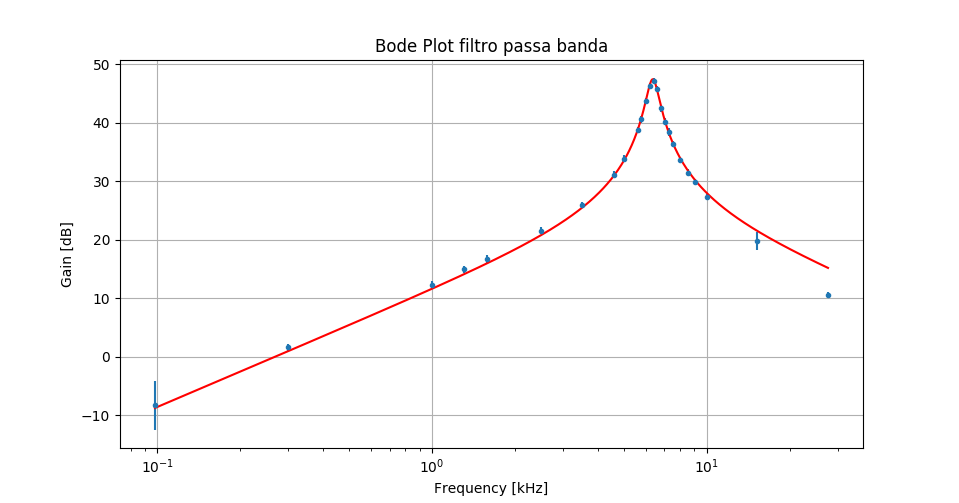
\includegraphics[scale=.7]{passabanda.png}
\caption{Fit del diagramma di Bode del circuito passa-banda.\label{bandaFit}}
\end{figure}

Ai fini di determinare solamente il guadagno massimo è stato eseguito un fit con un set di dati ridotto intorno al massimo della curva (figura \ref{bandaFitRidotta}). Esso da $A_2 = 234.9 \pm 1.2$, $f_0 = 6.349 \pm 0.002$kHz, $\Delta f = 638 \pm 6$Hz. La matrice di covarianza risulta essere: $ \Sigma_{ij} = \left( \begin{array}{ccc}
1.54 & -2.85 \cdot 10^{-4} & -6.19 \cdot 10^{-3}\\ 
-2.85 \cdot 10^{-4} & 5.12 \cdot 10^{-4} & 1.26 \cdot 10^{-6}\\
-6.20 \cdot 10^{-3} & 1.26 \cdot 10^{-6} & 3.43 \cdot 10^{-5}\\
\end{array} \right)$. Con un $\chi^2/ndof = 1/6$.\\

\begin{figure}[!htb]
\centering
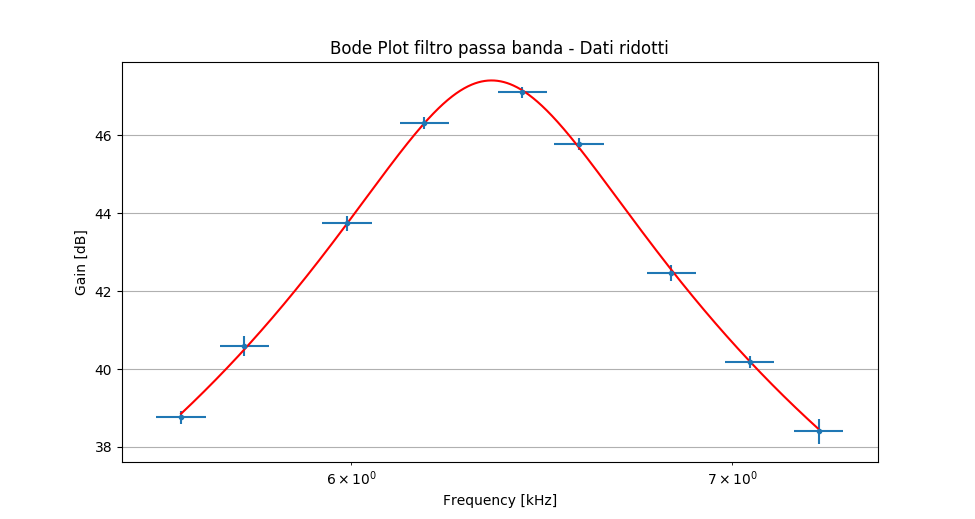
\includegraphics[scale=.7]{passaBandaRidotto.png}
\caption{Fit del diagramma di Bode del circuito passa banda - Centro banda.\label{bandaFitRidotta}}
\end{figure}


In conclusione l'amplificazione totale del circuito a centro banda, ottenuta moltiplicando i guadagni di tutti gli amplificatori misurati è: $A_0 = A_1 A_2 = (1.78 \pm 0.03) \cdot 10^5$, qui riportata perché usata nei calcoli seguenti.

\subsection{Convertitore RMS}
L'ultima parte del circuito ha lo scopo di trasformare un segnale alternato in un segnale continuo restituendone il valore quadratico medio ed è stato realizzato con l'apposito integrato nel circuito riportato in figura \ref{rmsCircuito}.

\begin{figure}[!htb]
\centering
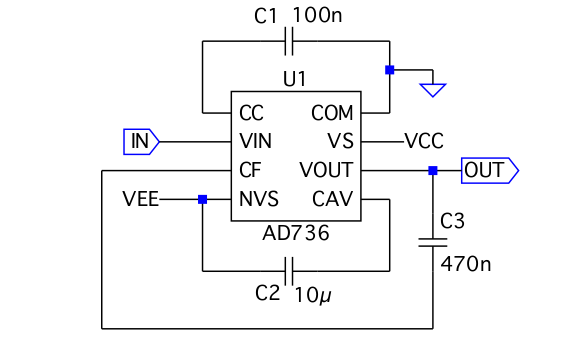
\includegraphics[scale=0.5]{rms.png}
\caption{Circuito RMS realizzato con appostito integrato.\label{rmsCircuito}}
\end{figure}

Inviando un segnale sinusoidale di ampiezza $V_{in} = 174 \pm 4$mV ci aspettiamo un segnale in uscita continuo $V_{out, att} = 123 \pm 3$mV, in ottimo accordo con quello misurato $V_{out, mis} = 124 \pm 4$mV. In  figura \ref{rms} si osservano il segnale in ingresso sinusoidale e il suo valore quadratico medio. Abbiamo verificato che entro il range di frequenze $500 \mbox{Hz} - 10 \mbox{kHz}$ il sistema funziona bene come RMS, ma al di fuori di questo no. La banda passante del passa-banda è ampiamente contenuta in questo range dunque questa limitazione non è un problema.

\begin{figure}[!htb]
\centering
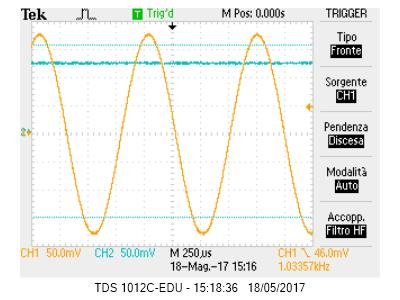
\includegraphics[scale=1.0]{vrms.jpg}
\caption{Verifica del funzionamento del circuito RMS.\label{rms}}
\end{figure}

\section{Misura della costante di Boltzmann}

Il rumore ($V_{rms})$ totale è determinato dalla somma in quadratura dei rumori associati alla resistenza e quelli dovuti all'amplificatore, parametrizzati come rumori in serie e in parallelo all'amplificatore. Dalla teoria ci aspettiamo dunque 
\begin{equation}
V_{rms} = V_0 \sqrt{1+\frac{R}{R_t}+(\frac{R}{R_n})^2}
\end{equation}
dove:
\begin{itemize}
\item $V_0$ è il rumore in uscita a resistenza nulla (dato solo dal rumore in serie all'amplificatore).
%non dovrebbe essere il rumore dell'amplificatore?
\item $R_t = \frac{V_0^2}{4 k_b T A_0^2 \Delta f}$ è la resistenza equivalente del rumore in serie sull'ingresso dell'amplificatore (resistenza che genererebbe un rumore termico equivalente). Il parametro $A_0$ è l'amplificazione totale del circuito utilizzato (misurata), $\Delta f$ è la larghezza di banda del circuito (a cui si suppone contribuisca solo il passa-banda), $T$ è la temperatura ambiente.\\
\item $R_n$ è il rapporto tra il rumore in parallelo e il rumore in serie dell'amplificatore. E' chiaro che il rumore in parallelo (a differenza del rumore in serie) è presente solamente se vi è una resistenza ai capi dell'ingresso dell'amplificatore.%Casi resitenza infinta e nulla non tonano proprio ma non scrivere (?) che cacchio ho scritto?
\end{itemize}

Le misure sono state eseguite misurando la tensione in uscita dal convertitore RMS con il multimetro digitale in DC. Si è visto che il valore misurato presentava forti oscillazioni e si è preso come errore sulla misura la semidispersione dei valori visualizzati dal multimetro e come misura la media di essi.
%qi forse ci cazziano perchè era meglio usare l'oscillo, ma vabbè abbiamo usato il multimetro quindi amen

In tabella \ref{bodeEstesi} e in figura \ref{boltzmannEsteso} sono riportati i valori di $V_{rms}$ per un range di resistenze che va da $1.78\mbox{k}\Omega$ a $216\mbox{k}\Omega$. Per resistenze di valore superiore i dati sono risultati essere totalmente inaffidabili: in particolare non si osservava più una dipendenza apprezzabile di $V_{rms}$ dal valore della resistenza.

%TODO Dire perch erano totalmente affidabili. Sopra i 100 ballano un sacco ma per resistenze veramente alte ho saturazione a un valore costante. Che cippa succede nel mezzo? Come è l'andamento di raccordo? non lo sappiamo

\begin{table}[!htb]\centering
\begin{tabular}{|c|c|c|c|}
\hline
$R (\mbox{k}\Omega)$ & $\Delta R (\mbox{k}\Omega)$ & $V_{rms} (mV)$ & $\Delta V_{rms} (mV)$\\
\hline
1.78 & 0.02 & 80 & 5\\
8.16 & 0.08 & 90 & 5\\
10.0 & 0.2 & 100 & 5\\
15.1 & 0.2 & 107 & 5\\
21.4 & 0.3 & 110 & 5\\
46.3 & 0.5 & 140 & 5\\
55.7 & 0.5 & 145 & 5\\
*80.8 & 0.7 & 175 & 10\\
*99.2 & 0.9 & 180 & 10\\
*118 & 2 & 215 & 10\\
*147 & 2 & 220 & 10\\
*216 & 3 & 230 & 10\\
\hline
\end{tabular}
\caption{Misure di $V_{rms}$ e relative resistenze.}
\label{bodeEstesi}
\end{table}

\begin{figure}[!htb]
\centering
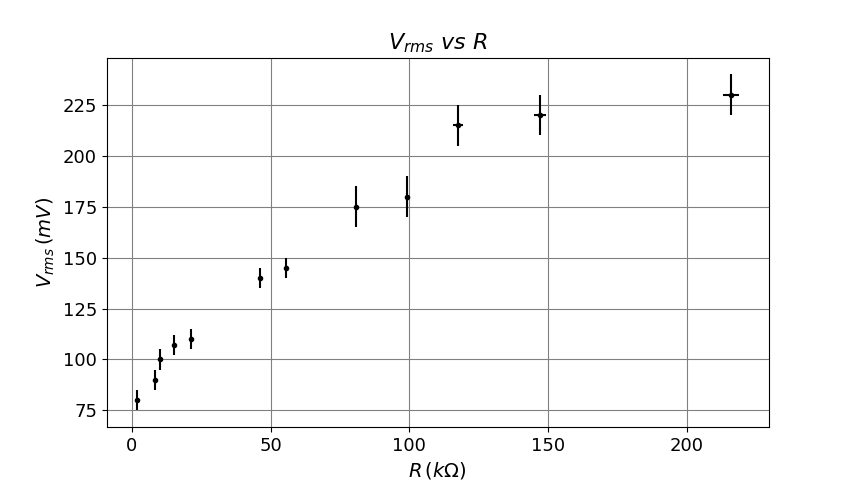
\includegraphics[scale=0.7]{boltzmannEsteso.png}
\caption{Plot di tutti i dati misurati $V_{rms}$ vs $R$.\label{boltzmannEsteso}}
\end{figure}

Si è eseguito inizialmente un fit a tre parametri della funzione $V_{rms} = V_0 \sqrt{1+\frac{R}{R_t}+(\frac{R}{R_n})^2}$. Il parametro $R_n$ risultava tuttavia essere dell'ordine delle decine di $\mbox{M}\Omega$ dunque l'ultimo termine si può considerare ininfluente. In effetti $R_n$ restituito dall'algoritmo di fit fluttuava anche di un ordine di grandezza al variare del valore iniziale dal quale si esegue la minimizzazione del $\chi^2$. Per questi motivi il fit è stato ripetuto a due parametri: $V_{rms} = V_0 \sqrt{1+\frac{R}{R_t}}$.
\\
%TODO non capisco qua perchè non hai messo i risultati del fit!
Nel successivo fit sono stati escluse le righe marcate con l'asterisco nella tabella \ref{bodeEstesi} poiché affetti da fluttuazioni troppo grandi come si può vedere dagli errori\footnote{Alla procedura di fit sono stati forniti solo gli errori sulle tensioni e non quelli sulle resistenze in quanto trascurabili nella regione di dati usata.}.

%Ho scritto come si propagano gli errori... In quadratura. 
I parametri riportati dal fit sono $V_0 = 80 \pm 3$mV e $R_t = 23 \pm 3 \mbox{k}\Omega$. La matrice di covarianza è:  $\Sigma_{ij} = \left( \begin{array}{cc}
12.1 & 11.8\\ 
11.8 & 13.9\\
\end{array} \right)$. Con un $\chi^2/ndof = 2.76/5$ (basso per probabile sovrastima delle incertezze).\\
Invertendo la formula per $R_t$ otteniamo: $k_B = \frac{V_0^2}{4 R_t T A_0^2 \Delta f}=(1.43 \pm 0.14) \cdot 10^{-23} \frac{J}{K}$. La temperatura è stata stimata (arbitrariamente) come $T = 298 \pm 2$K. Gli errori più significativi che si propagano (in quadratura) in questa formula sono quelli sui parametri del fit della curva di rumore.
%TODO dire che abbiamo preso come tempertura 28 gradi (mi pare) e mettiamoci un più o meno 3  gradi di incertezza direi... diciamo stima arbitraria?
%A rigore la propagazione in qudratura è sbagliata per la temp. ma per gli altri è giusta.

\begin{figure}[!htb]
\centering
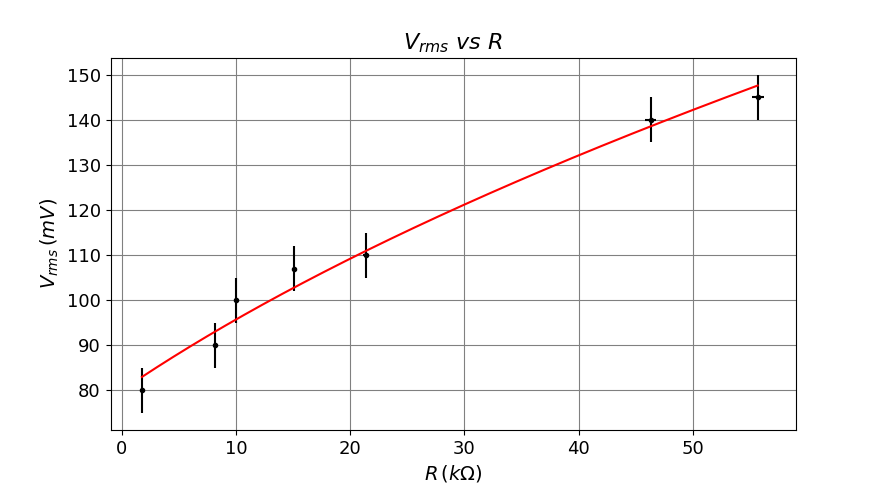
\includegraphics[scale=0.7]{boltzmann.png}
\caption{Fit $V_{rms}$ vs $R$ con i dati più stabili.\label{boltzmannFit}}
\end{figure}

Di seguito (figura \ref{boltzEstesi}) è riportato il fi eseguito con tutti i dati nella tabella \ref{bodeEstesi}.

\begin{figure}[!htb]
\centering
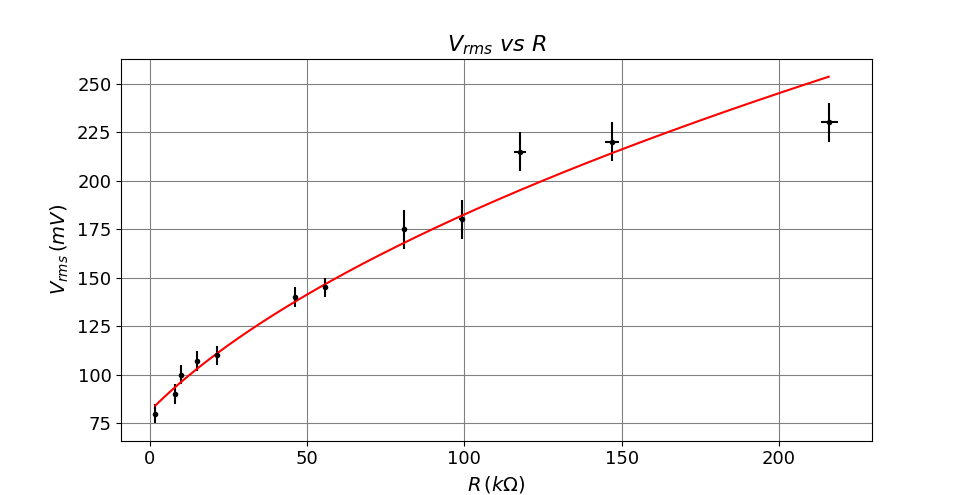
\includegraphics[scale=0.7]{boltzmannEstesoFit.png}
\caption{Fit $V_{rms}$ vs $R$ con tutti i dati.\label{boltzEstesi}}
\end{figure}

I parametri estratti (e non utilizzati) sono $V_0 = 81 \pm 3$mV e $R_t = 24 \pm 3 \mbox{k}\Omega$. La matrice di covarianza è:  $\Sigma_{ij} = \left( \begin{array}{cc}
8.80 & 7.76\\ 
7.56 & 7.48\\
\end{array} \right)$. Con $\chi^2/ndof = 13/10$.

%TODO Forse in effetti sarebbe meglio usare questi dati che sembrano avere meno errore, in barba a quello che avevo detto prima.

Il valore atteso della costante di Boltzmann è $k_{B} = 1.38 \cdot 10^{-23} \frac{J}{K}$. Il valore da noi misurato è ragionevolmente in accordo con esso.

\end{document}







